\chapter{Background and Literature Review}
\label{ch:background}
\section{GPS Overview}

Chapter~\ref{chapter:introduction} introduced LAAS, which is based on the Global Positioning System developed by the U.S. Department of Defense (DOD).  GPS is a remarkable system for finding one's location and its success is largely due to the modest needs of the average user. Standard GPS accuracy is approximately 15 meters\citep[]{GPS_FOR_DUMMIES} and this level of accuracy is quite satisfactory for many applications, including land navigation, which is the primary consumer application for GPS. However, when GPS accuracy is discussed it is generally in terms of horizontal accuracy.  Vertical accuracy is seldom mentioned in the discussion of accuracy and most GPS manufacturers do not publish the vertical accuracy specification.  Due to this, a rule-of-thumb has developed that suggests that the vertical accuracy is only half as good as the horizontal accuracy.  So, if Standard GPS is accurate to within 15 meters in the horizontal, then it is considered accurate to about 30 meters in the vertical, which is unacceptable for aircraft landings. This is why LAAS is indispensable for a GPS Landing System (GLS).  Many different factors affect the precision of GPS which will be explored during this overview of the Global Positioning System.

GPS is comprised of 24 well placed satellites. The satellites orbit the earth in 6 orbital planes that are at a 55$^o$ inclination with 4 satellites per plane such that at least 4 satellites will be above the horizon at any given moment. This allows users the ability to use the system 24 hours a day anywhere on the planet. These satellites are not geo-orbital, but are at a Medium Earth Orbit (MEO) and orbit the earth twice a sidereal day with a speed of 3.9km per second.  The basic principal of the GPS system is quite simple.  A satellite orbits the earth at about 12,600 miles shown in Figure~\ref{fig:GPS_Basics_1}. The satellite acts as a reference point with a known distance which is called its \textit{range}.  How this range is known will be discussed later, but for now the user receiver knows one thing, that it lies on a sphere centered at the satellite with a known radius.

\begin{figure}
  \centering
	\scalebox{.9}{
	\mbox{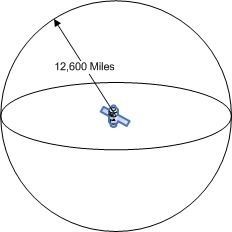
\includegraphics{figures/GPS_Basics_1.jpg}}
	}
  \caption{GPS Basics: Radius}
	\label{fig:GPS_Basics_1}
\end{figure}

If two satellite are used then this narrows the possible location down to the circle where the two spheres centered at each satellite intersect, shown in Figure~\ref{fig:GPS_Basics_2}. When a third satellite is introduced it intersects the circle at two points shown in Figure~\ref{fig:GPS_Basics_3}. Purely speaking a fourth measurement should be used to unambiguously locate a point in space, but for GPS this is not the case.  Of the two points referenced, one is normally a sensible answer and the other is either not located on Earth or is moving at an unreasonable velocity (measured in the range of thousands of kilometers per second).

\begin{figure}
	\centering
	\scalebox{.5}{
	\mbox{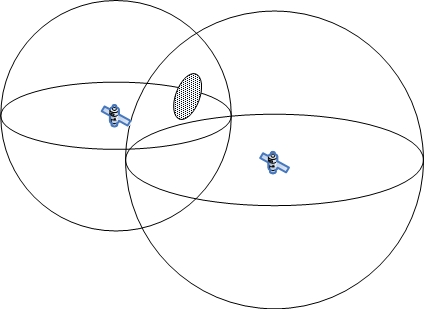
\includegraphics{figures/GPS_Basics_2.jpg}}
	}
	\caption{GPS Basics: Circle}
	\label{fig:GPS_Basics_2}
\end{figure}


\begin{figure}
	\centering
	\scalebox{.55}{
	\mbox{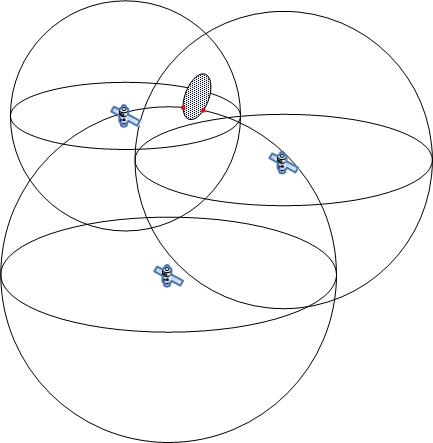
\includegraphics{figures/GPS_Basics_3.jpg}}
	}
	\caption{GPS Basics: Two Points}
	\label{fig:GPS_Basics_3}
\end{figure}

The satellites are used as reference points, but how can something moving high above the earth at a high velocity be used for measuring distance?  Every aspect of the GPS constellation is precisely monitored by six earth based monitor stations located throughout the world.  Any variance in the orbit, position, or velocity of a satellite is compensated and adjusted for at the master control station, located in Colorado Springs, Colorado.  These constant adjustments are put into a GPS message called the ephemeris message.  An \textit{ephemeris} is a table giving the coordinates of a set of celestial bodies at a number of specific times during a given period.  This data allows a GPS receiver to know the exact position of a satellite at a given time.  Now a method similar to \textit{trilateration} can be used to determine the GPS receiver's range or distance to the satellite. Trilateration uses the known locations of three or more reference points, and the measured distance between the subject and each reference point to determine the subject's location. In the case of GPS the distance is measured using the time-of-arrival (TOA) of a ranging signal called the \textit{pseudorandom code} (PRN). The code is a very complex set of digital information that is called pseudorandom because it resembles random noise. It is repeated every millisecond. When the receiver receives the pseudorandom code it takes the signal propagation time multiplied by the speed of light to get the range to the satellite.  This is simple in concept, but the timing has to be near perfect.  If the time is off by even 1/1000 of a second the range could be off by 300,000 meters.  The satellites actually keep track of time using atomic clocks.  Each satellite is equipped with four atomic clocks to precisely track time, but atomic clocks are very costly and impractical for producing low cost GPS receivers.  Instead manufacturers use a less precise, less expensive crystal clock; but now have to overcome the error introduced by the receiver clock. Thus time becomes a fourth unknown. This is resolved with an additional satellite measurement. If three measurement made with perfect time can be used to produce a position solution then four inexact measurements can be used to produce the same solution while solving for the receiver clock offset.  Once the receiver's clock has been adjusted then not only will the receiver produce an accurate position, but it also works as a functional atomic clock.  Theses techniques provide a more accurate range to satellites, but these ranges still contain errors; therefore they are referred to as \textit{pseudoranges}.  The errors can be categorized as follows:

\begin{itemize}
	\item Ephemeris ($<$ 1 meter Error)

As mentioned earlier an ephemeris is a table of the coordinates of a celestial body at a point in time. This of course uses a model to predict where the satellite will be, but the forces acting upon the satellite don't always conform perfectly to the model which does introduce some error.  Since the ephemeris data is constantly being adjusted the error introduced is small and can be removed by differential GPS between two observations of short separation.

	\item Satellite Clock Errors ($<$ 1 meter Error)

Satellites use atomic clocks to precisely monitor time, but even atomic clocks are not perfect.  Since the pseudorange calculation is based on time any discrepancy in the clock will introduce error.  This can also be removed with differential GPS.

	\item Receiver Clock Errors (1 meter $<$ Error $<$ 2 meters)

A GPS Receiver uses a crystal clock which is much less accurate than an atomic clock; consequently additional timing errors exist.  The Receiver Clock produces more error than the Satellite Clock and unfortunately can not be removed with differential GPS, but is treated as another unknown during the estimation process.

	\item Ionosphere / Troposphere ($\approx$4 meters)

The atmosphere can be broken down into many layers but the two that most affect GPS are the Ionosphere and the Troposphere.  The Ionosphere is a dispersive medium, therefore the GPS signal is bent and changes speed as it passes through the ionosphere. Though the bending is generally negligible, the ionosphere increases the speed of the carrier phase and slows down the pseudorandom code, so this source of error must be taken into consideration.  The troposphere, on the other hand, is a non dispersive medium, so the carrier phase and pseudorandom code are delayed by the same amount increasing the measured distance to the satellite from the actual distance.\cite[]{EL-RABBANY}.

 	\item GPS Satellite Geometry

A Satellite's geometry with respect to other satellites also plays a role in the position solution.  The closer the satellites are to one another the poorer the position solution and the more spread out the better the position solution.  The Dilution of Precision (DOP) is a number that represents the acceptability of the GPS geometry.  It can further be broken down into a horizontal and vertical component known as the Horizontal Dilution of Precision (HDOP) and Vertical Dilution of Precision (VDOP).

	\item Multipath

Multipath is a source of error that is introduced when the GPS signal is received by the GPS receiver from different paths; one signal may take the direct path and another signal be reflected off of some structure. This is the same occurrence that causes ghosting on a television set. LAAS reduces the potential of this error source by using specialized GPS Multipath Limiting Antennas (MLA) and a priori siting analysis to avoid multipath generating structures.

	\item Selective Availability (SA) ($>$ 10 Meters)

The last error that will be mentioned is artificial error.  The U.S. Military purposely skewed the GPS signal to artificially inflate the error in the system so that it could not be used against them.  When Selective Availability was active it was the most substantial source of error, but the use of differential GPS could nearly eliminate SA's effectiveness. The use of SA was discontinued on May 1, 2000.

\end{itemize}

\section{Differential GPS (DGPS)\label{section:DGPS}}

Differential GPS is the method of using a GPS receiver at a fixed known reference point to determine the errors in GPS ranging. To do this, the GPS receiver's antenna position is accurately surveyed.  Next, the difference is calculated between the pseudorange internally measured by the GPS receiver and the pseudorange calculated from a satellite's current GPS almanac, ephemeris information, and the surveyed location.  The difference between the measured pseudorange and the calculated pseudorange is the \textit{pseudorange correction} which is the distance that the local user should adjust a respective satellite's pseudorange by to achieve a minimum error position solution. The pseudorange correction is a lump sum adjustment for multiple sources of error which include ephemeris, satellite and receiver clocks, ionosphere and troposphere, and even Selective Availability. However, the pseudorange correction can only be computed by knowing the precise location of the reference receiver antenna. Another thing to note is that most Differential GPS systems make corrections in the range domain by adjusting the pseudorange measurement of each satellite in view.  An alternative approach is to adjust the system in the position domain.  This would involve calculating a position solution for the reference point then calculating a position correction vector.  This is generally not done due to the fact that position solutions are calculated by manufacturers using proprietary methods, and their behavior is not known a priori.

The many different Differential GPS solutions that have been developed fall broadly into two categories: post-processed and real time. Surveyors are a primary user of the non-real time post-processing category.  They collect GPS data from known reference points, which they call \textit{benchmarks}, and the point needing to be surveyed.  The distance between the benchmark and the survey point is called the \textit{baseline}, and it is generally preferred to use the benchmark with the shortest baseline to the survey point. After about 15 minutes to an hour of collecting data at both locations they can post process the data with GPS utilities to produce a position solution accurate to within a centimeter\footnote{Utilizes GPS L1/L2 survey equipment}.  On the other hand, real-time differential GPS systems acquire the data from the reference points, calculate the pseudorange corrections, and broadcast them out at a rate of 2 to 5 Hertz to be used in navigation applications. Since LAAS falls into the real time category, it and a few other prominent real time DGPS systems will be discussed.

One of the first systems developed actually used the acronym DGPS, but sometimes also goes by NDGPS (Nationwide Differential Global Positioning System) to distinguish DGPS the concept from DGPS the system.  The NDGPS is used by the U.S. Coast Guard in harbor regions to give ships better position solutions.  Even though the name implies national coverage is it limited to coastal regions. Europe and Canada also have similar solution for their heavily utilized maritime locations. There are even commercial companies like VERIPOS, StarFire, and OmniSTAR that provide Differential GPS services.

\begin{figure}
	\centering
	\scalebox{1.437}{
	\mbox{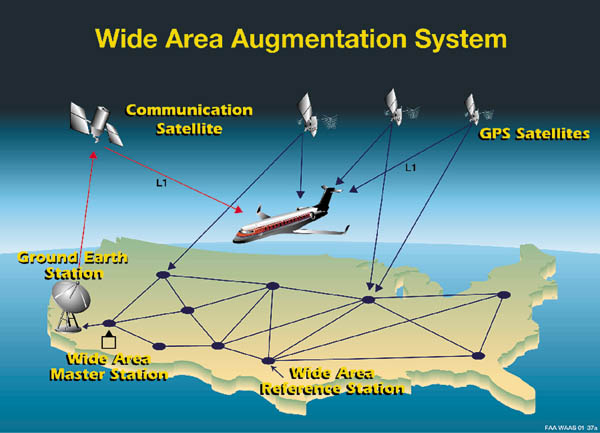
\includegraphics{figures/waas.jpg}}
	}
	\caption{Wide Area Augmentation System\citep[]{FAA_WAAS}}
	\label{fig:FAA_WAAS}
\end{figure}

Most of the DGPS systems developed had a very specific function or operated in such a localized area that it precluded widespread use. The FAA wanted to capitalize on the benefits of DGPS while promoting a broad coverage area. To that end they designed the Wide Area Augmentation System.  WAAS, as shown in Figure~\ref{fig:FAA_WAAS}, established reference points throughout the contiguous United States. These fixed reference points were used to establish pseudorange corrections for most of North America.  The WAAS corrections are then sent to a geo-orbital satellite and broadcast to WAAS-enabled GPS receivers.  WAAS improved the accuracy of GPS to less than 2 meters in the horizontal and less than 3 meters in the vertical. This was a significant enhancement to GPS; an improved GPS position solution free for the end user.  GPS manufacturers adopted this readily and now WAAS-enabled GPS receivers are commonplace. A major shortcoming with WAAS is its confinement to North America.  Additional Reference Receivers are being installed in Alaska and Mexico, but this is still a United States / North America locale. Large air carriers need GPS augmentation internationally. Furthermore, WAAS accuracy is not as accurate as some other Differential GPS systems due to its broad coverage area.  Because of this the FAA does not consider its accuracy and integrity acceptable for instrument landings beyond CAT I.

\begin{figure}
	\centering
	\scalebox{.907}{
	\mbox{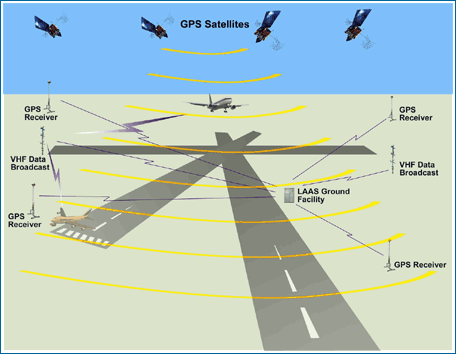
\includegraphics{figures/LAAS_Architecture.png}}
	}
	\caption{Local Area Augmentation System\citep[]{FAA_LAAS}}
	\label{fig:FAA_LAAS}
\end{figure}

The Local Area Augmentation System was initiated by the FAA to provide an accurate real time differential GPS solution . The LAAS concept follows that of WAAS, but the reference receivers are generally located within the airport environment as can be seen in Figure~\ref{fig:FAA_LAAS}.  Further, the differential GPS corrections are only usable within the VDB broadcast range, which is about 20 to 30 miles.  By limiting the operating region LAAS is able to deliver accuracy under 1 meter in both the horizontal and vertical axis\cite[]{FAA_LAAS}. A further benefit is that LAAS is only dependent on the GPS fleet; therefore it can be used anywhere in the world.  The FAA formalized the interfaces and many of the algorithms that should be used in a LGF. Components of a software architecture for a Local Area Augmentation System will be examined in the remainder of this thesis, including the host architecture, message formats, and message broadcasting.

\begin{table}[htbp]
    \centering
    \caption{WAAS Sites}
\resizebox{\columnwidth}{!}{
\begin{tabular}{ l l l l l}
\hline
\textbf{City} &
\textbf{ICAO airport code} &
\textbf{Antenna 1} &
\textbf{Antenna 2} &
\textbf{Antenna 3}\\ \hline
Bethel, Alaska                           & PABE     & 60.787916486°N 161.841724416°W, 52.203 m    & 60.787897064°N 161.841663857°W, 52.204 m    & 60.787881127°N 161.841728605°W, 52.198 m\\
Billings, Montana                        & KBIL     & 45.803707088°N 108.539722283°W, 1112.261 m  & 45.803716383°N 108.539780649°W, 1112.266 m  & 45.803756811°N 108.539680968°W, 1112.255 m\\
Barrow, Alaska                           & PABR     & 71.282765883°N 156.789923397°W, 15.577 m    & 71.282798595°N 156.789965306°W, 15.589 m    & 71.282793925°N 156.789856228°W, 15.577 m\\
Cold Bay, Alaska                         & PACD     & 55.200334771°N 162.718472052°W, 53.648 m    & 55.200394330°N 162.718489390°W, 53.652 m    & 55.200400493°N 162.718623936°W, 53.657 m\\
Fairbanks, Alaska                        & PAFA     & 64.809630987°N 147.847339789°W, 149.891 m   & 64.809681435°N 147.847491409°W, 149.897 m   & 64.809748030°N 147.847379206°W, 149.876 m\\
Honolulu, Hawaii                         & PHNL     & 21.312988930°N 157.920824884°W, 24.678 m    & 21.312645960°N 157.920980760°W, 25.022 m    & 21.312714586°N 157.920825156°W, 25.067 m\\
Juneau, Alaska                           & PAJN     & 58.362575024°N 134.585705943°W, 16.024 m    & 58.362469451°N 134.585487326°W, 16.029 m    & 58.362545895°N 134.585292259°W, 16.020 m\\
Mérida, Yucatán                          & MMMD     & 20.931909130°N 089.662840352°W, 29.133 m    & 20.931901399°N 089.662887739°W, 29.171 m    & 20.931946482°N 089.662890840°W, 29.168 m\\
Mexico City                              & MMMX     & 19.431653203°N 099.068389471°W, 2236.638 m  & 19.431676477°N 099.068348099°W, 2236.625 m  & 19.431629899°N 099.068430820°W, 2236.652 m\\
Puerto Vallarta, Jalisco                 & MMPR     & 20.679003359°N 105.249202871°W, 10.973 m    & 20.679041461°N 105.249177972°W, 11.269 m    & 20.679059454°N 105.249221363°W, 10.990 m\\
San José del Cabo, Baja California Sur   & MMSD     & 23.160445938°N 109.717646195°W, 104.297 m   & 23.160383141°N 109.717652895°W, 104.285 m   & 23.160419201°N 109.717704568°W, 104.277 m\\
Tapachula, Chiapas                       & MMTP     & 14.791366074°N 092.367999089°W, 54.962 m    & 14.791334042°N 092.367965119°W, 54.950 m    & 14.791319966°N 092.368009440°W, 54.855 m\\
Kotzebue, Alaska                         & PAOT     & 66.887333160°N 162.611372024°W, 10.911 m    & 66.887368005°N 162.611390215°W, 10.909 m    & 66.887356742°N 162.611304386°W, 10.913 m\\
Iqaluit, Nunavut                         & CYFB     & 63.731490169°N 068.543181586°W, 10.022 m    & 63.731464001°N 068.543402553°W, 9.957 m     & 63.731386362°N 068.543596671°W, 10.014 m\\
Gander, Newfoundland and Labrador        & CYQX     & 48.966489496°N 054.597631164°W, 146.888 m   & 48.966447606°N 054.597532034°W, 146.887 m   & 48.966406383°N 054.597433025°W, 146.899 m\\
Winnipeg, Manitoba                       & CYWG     & 49.900574663°N 097.259396222°W, 222.042 m   & 49.900677586°N 097.259217224°W, 222.051 m   & 49.900568446°N 097.259226893°W, 222.045 m\\
Goose Bay, Newfoundland and Labrador     & CYYR     & 53.308646665°N 060.419467188°W, 37.830 m    & 53.308713007°N 060.419365697°W, 37.844 m    & 53.308803193°N 060.419371104°W, 37.853 m\\
Albuquerque, New Mexico                  & KZAB     & 35.173575457°N 106.567349162°W, 1620.117 m  & 35.173574799°N 106.567287780°W, 1620.181 m  & 35.173532365°N 106.567287878°W, 1620.164 m\\
Anchorage, Alaska                        & PAZA     & 61.229202467°N 149.780248917°W, 80.660 m    & 61.229118812°N 149.780422686°W, 80.653 m    & 61.229202391°N 149.780423003°W, 80.648 m\\
Aurora, Illinois                         & KZAU     & 41.782657876°N 088.331335953°W, 195.918 m   & 41.782595526°N 088.331334442°W, 195.921 m   & 41.782596464°N 088.331253756°W, 195.926 m\\
Nashua, New Hampshire                    & KZBW     & 42.735720140°N 071.480425027°W, 39.125 m    & 42.735724128°N 071.480358015°W, 39.151 m    & 42.735671312°N 071.480352294°W, 39.147 m\\
Leesburg, Virginia                       & KZDC     & 39.101595603°N 077.542745736°W, 80.084 m    & 39.101523590°N 077.542730286°W, 80.080 m    & 39.101548982°N 077.542774296°W, 80.092 m\\
Longmont, Colorado                       & KZDV     & 40.187303318°N 105.127223496°W, 1541.399 m  & 40.187303552°N 105.127154188°W, 1541.391 m  & 40.187253096°N 105.127167214°W, 1541.377 m\\
Fort Worth, Texas                        & KZFW     & 32.830649739°N 097.066471191°W, 155.617 m   & 32.830596303°N 097.066523654°W, 155.576 m   & 32.830598335°N 097.066470282°W, 155.620 m\\
Houston, Texas                           & KZHU     & 29.961896297°N 095.331425748°W, 10.908 m    & 29.961831785°N 095.331449752°W, 10.974 m    & 29.961773563°N 095.331512004°W, 10.958 m\\
Hilliard, Florida                        & KZJX     & 30.698859379°N 081.908184568°W, 2.149 m     & 30.698823791°N 081.908152480°W, 2.140 m     & 30.698791217°N 081.908198025°W, 2.135 m\\
Olathe, Kansas                           & KZKC     & 38.880159315°N 094.790833106°W, 305.904 m   & 38.880160009°N 094.790643592°W, 305.903 m   & 38.880101810°N 094.790710614°W, 305.636 m\\
Palmdale, California                     & KZLA     & 34.603517830°N 118.083893947°W, 763.521 m   & 34.603517881°N 118.083828796°W, 763.520 m   & 34.603473855°N 118.083893956°W, 763.598 m\\
Salt Lake City, Utah                     & KZLC     & 40.786043564°N 111.952176782°W, 1287.421 m  & 40.785990178°N 111.952176149°W, 1287.416 m  & 40.785990067°N 111.952122320°W, 1287.423 m\\
Miami, Florida                           & KZMA     & 25.824611968°N 080.319189364°W, -7.579 m    & 25.824659706°N 080.319315758°W, -8.207 m    & 25.824661752°N 080.319234381°W, -7.861 m\\
Memphis, Tennessee                       & KZME     & 35.067394005°N 089.955369299°W, 68.609 m    & 35.067437537°N 089.955368937°W, 68.883 m    & 35.067439374°N 089.955436864°W, 68.871 m\\
Farmington, Minnesota                    & KZMP     & 44.637463181°N 093.152084552°W, 262.679 m   & 44.637463059°N 093.152011267°W, 262.693 m   & 44.637407004°N 093.152022108°W, 262.628 m\\
Ronkonkoma, New York                     & KZNY     & 40.784328238°N 073.097164869°W, 6.457 m     & 40.784275495°N 073.097154931°W, 5.930 m     & 40.784275925°N 073.097223653°W, 5.936 m\\
Fremont, California                      & KZOA     & 37.543053122°N 122.015945899°W, -3.497 m    & 37.543025498°N 122.015892540°W, -3.481 m    & 37.542981164°N 122.015929270°W, -3.400 m\\
Oberlin, Ohio                            & KZOB     & 41.297154278°N 082.206443927°W, 223.689 m   & 41.297166589°N 082.206351733°W, 225.187 m   & 41.297086827°N 082.206379312°W, 223.468 m\\
Auburn, Washington                       & KZSE     & 47.286993478°N 122.188372098°W, 82.112 m    & 47.286907917°N 122.188382169°W, 82.168 m    & 47.286856213°N 122.188363949°W, 82.105 m\\
San Juan, Puerto Rico                    & TJZS     & 18.431335686°N 065.993476761°W, -28.062 m   & 18.431218583°N 065.993514086°W, -28.047 m   & 18.431198889°N 065.993448100°W, -28.108 m\\
Hampton, Georgia                         & KZTL     & 33.379688402°N 084.296725378°W, 261.138 m   & 33.379691546°N 084.296656313°W, 261.126 m   & 33.379634831°N 084.296652682°W, 261.161 m\\
\end{tabular}
}
\label{tab:WAAS_SITES}
\end{table}
